\chapter{Penggunaan ABS MVC Framework}

Bab ini membahas tentang penggunaan ABS MVC Framework dalam pengembangan perangkat lunak berbasis web.

\section{Gambaran Umum Aplikasi Web}
Aplikasi web yang akan dibuat pada bab ini adalah aplikasi katalog produk yang fungsinya adalah untuk menyimpan dan menampilkan data tentang produk yang akan dijual di pasaran. Aplikasi web ini dibuat dengan tujuan untuk mendemonstrasikan tentang bagaimana membuat operasi \textit{create}, \textit{retrieve}, \textit{update} dan \textit{delete} (CRUD) dengan menggunakan ABS MVC Framework. Selain itu, penulis juga akan mendemonstrasikan bagaimana mengelola \textit{variability} degan pendekatan \textit{delta modelling} menggunakan ABS MVC Framework.\\

Berikut ini adalah fitur dari aplikasi web yang akan dibuat dengan menggunakan ABS MVC Framework:

\begin{enumerate}
    \item Menyimpan data produk (sku\footnote{\textit{stock keeping unit}, merupakan kode unik yang diberikan kepada setiap item sebagai bentuk identifikasi barang}, nama produk, deskripsi, harga).
    \item Menampilkan daftar produk.
    \item Mengubah data produk.
    \item Menghapus data produk.
\end{enumerate}

\section{Pembuatan Komponen Model}

Seperti yang sudah dibahas pada bab sebelumnya, komponen Model merupakan representasi dari data yang ada di dalam aplikasi. Dalam konteks aplikasi web yang akan dibuat, komponen Model ini akan merepresentasikan data produk yang yang akan disimpan oleh sistem dan ditampilkan kepada pengguna aplikasi. Pada tahap ini, penulis membuat sebuah modul ABS barus bernama \texttt{Product} dan menyimpan modul tersebut dengan nama \textit{Product.abs} di dalam direktori \texttt{src/abs/model} milik ABS MVC Framework.\\

Setelah selesai membuat modul baru, berikutnya adalah menuliskan kode ABS untuk mendefinisikan modul \texttt{Product} tersebut. Berikut ini adalah kode yang harus ditulis di dalam modul \texttt{Product}:

\begin{lstlisting}[
caption=Kode ABS untuk mendefinisikan komponen Model \texttt{Product},
label={lst:absProductModel},
escapeinside={@}{@}
]
module Model.Product;
export *;

interface Product
{
	String getSku(); @\label{lst:modelAccessor}@
	String getName();
	String getDescription();
	String getPrice();
	Unit setSku(String sku); @\label{lst:modelMutator}@
	Unit setName(String name);
	Unit setDescription(String description);
	Unit setPrice(String price);
}

class ProductImpl 
	(String sku, String name, String description, String price) implements Product
{
	String getSku() { return this.sku; }
	String getName() { return this.name; }
	String getDescription() { return this.description; }
	String getPrice() { return this.price; }
	Unit setSku(String sku) { this.sku = sku; }
	Unit setName(String name) { this.name = name; }
	Unit setDescription(String description) { this.description = description; }
	Unit setPrice(String price) { this.price = price; }
}
\end{lstlisting}

Seperti yang terlihat pada kode \ref{lst:absProductModel} di atas, konten dari \texttt{Product} hanya berisi atribut-atribut data seperti "sku", "name", "description", dan "price" beserta \textit{method} aksesor (\texttt{getSku()}) dan mutatornya (\texttt{setSku()}). Satu hal yang harus diperhatikan dalam mendefinisikan komponen Model ini adalah konvensi penamaan untuk \textit{method} aksesor dan mutatornya. Konvensi penamaan yang digunakan pada \textit{framework} ini adalah dengan memberikan prefix \texttt{set} untuk mutator dan \texttt{get} untuk aksesor yang kemudian diikuti dengan nama atribut dengan menggunakan format \textit{camel case} (lihat baris \ref{lst:modelAccessor} dan \ref{lst:modelMutator}). Konvensi ini ditujukan agar komponen Model yang dibuat dapat dikenali oleh Thymeleaf.\\

Setelah selesai membuat komponen Model, selanjutnya adalah membuat modul bantuan yang akan digunakan untuk mensimulasikan basis data pada aplikasi. Hal ini dilakukan karena ABS MVC Framework yang digunakan belum dapat mengakses basis data secara langsung seperti yang sudah disebutkan pada bagian batasan penelitian. Operasi-operasi yang dimiliki oleh modul ini antara lain adalah:

\begin{enumerate}
    \item \texttt{save}: operasi ini digunakan untuk menyimpan data produk yang diberikan.
    \item \texttt{delete}: operasi ini digunakan untuk menghapus data produk tertentu.
    \item \texttt{update}: operasi ini digunakan untuk mengubah data produk yang sudah tersimpan.
    \item \texttt{findAll}: operasi ini digunakan untuk mendapatkan seluruh data produk yang tersimpan.
    \item \texttt{findBySku}: operasi ini digunakan untuk mendapatkan data produk sesuai dengan kode SKU yang diberikan.
\end{enumerate}

Pada tahap ini penulis membuat sebuah modul baru yang bernama \texttt{ProductDB} yang kemudian disimpan ke dalam direktori \texttt{src/abs/model} dengan nama \texttt{ProductDB.abs}. Berikut ini adalah konten dari module \texttt{ProductDB.abs}:

\begin{lstlisting}[
caption=Kode ABS untuk modul \texttt{ProductDB},
label={lst:absProductDB},
escapeinside={@}{@}
]
module Model.ProductDB;
export *;
import Product, ProductImpl from Model.Product;

interface ProductDB
{
	Unit init();
	List<Product> findAll();
	Product findBySku(String sku);
	Unit save(Product obj);
	List<Product> delete(Product obj);
	List<Product> update(Product obj);
}

class ProductDBImpl implements ProductDB
{
	List<Product> db = Nil; @\label{lst:absProductList}@
	
	Unit init() @\label{lst:absProductDBInit}@
	{
		Product p1 = new local ProductImpl(
			"WH001", "LED TV 24' ", "FMSE LED TV 24 inch with 2 HDMI", "2.500.000");
			
		Product p2 = new local ProductImpl(
			"WH002", "LED TV 24' ", "FMSE LED TV 24 inch with 2 HDMI", "4.500.000");
			
		Product p3 = new local ProductImpl(
			"WH003", "Rice Cooker", "FMSE Electric Rice Cooker 5 litre", "1.500.000");
			
		db = appendright(db, p1);
		db = appendright(db, p2);
		db = appendright(db, p3);
	}
	
	List<Product> findAll()
	{
		return db;
	}
	
	Product findBySku(String sku)
	{
		Product result = null;
		Int index = 0;
		
		while(index < length(db))
		{
			Product current = nth(db, index);
			String currentSku = current.getSku();
			
			if(currentSku == sku)
			{
				result = current;
			}
			
			index = index + 1;	
		}
		
		return result;
	}
	
	Unit save(Product obj)
	{
		db = appendright(db, obj);
	}
	
	List<Product> delete(Product obj)
	{
		db = without(db, obj);
		
		return db;
	}
	
	List<Product> update(Product obj)
	{
		db = without(db, obj);
		db = appendright(db, obj);
		
		return db;
	}
}
\end{lstlisting}

Seperti yang terlihat pada kode \ref{lst:absProductDB} baris \ref{lst:absProductList} diatas, penulis membuat sebuah \texttt{List<Product>} yang digunakan untuk menyimpan seluruh data produk. Setiap operasi-operasi yang ada di dalam modul \texttt{ProductDB} ini nantinya akan menggunakan \texttt{List<Product>} tersebut sebagai sumber datanya.\\

Untuk keperluan pengembangan aplikasi web yang dibuat, penulis membuat tiga buah data \textit{dummy} sebagai data awalan yang kemudian dimasukan kedalam \texttt{List<Product>} yang telah dibuat. Data awalan tersebut dibuat di dalam sebuah \textit{method} khusus bernama \textit{init} (lihat kode \ref{lst:absProductDB} baris \ref{lst:absProductDBInit}) yang akan dipanggil setiap kali melakukan inisialisasi modul ini. Dengan menggunakan pendekatan ini, penulis dapat mensimulasikan proses \textit{create}, \textit{retrieve}, \textit{update} dan \textit{delete} pada aplikasi web yang dibuat.

\section{Pembuatan Komponen View}

Setelah selesai membuat komponen Model, langkah berikutnya adalah membuat komponen View. Pada pengembangan aplikasi web ini, terdapat empat buah halaman HTML yang menjadi komponen View-nya. Keempat halaman tersebut harus disimpan kedalam folder \texttt{src/abs/view/product} agar dapat dikenali oleh ABS MVC Framework. Berikut ini adalah daftar berkas HTML yang harus dibuat berikut dengan kodenya:

\subsection{Komponen View \texttt{index.html}}
Halaman HTML ini berfungsi sebagai halaman depan aplikasi yang berisikan informasi gambaran umum sistem dan cara penggunaannya. berikut ini adalah kode HTML yang harus dimasukan kedalam berkas \texttt{index.html} beserta gambar halaman web yang akan ditampilkan:

\begin{lstlisting}[
caption=Kode HTML untuk halaman \texttt{index.html},
label={lst:htmlIndex}
]
<!DOCTYPE html>
<html>
	<head>
		<title>Aplikasi Katalog Produk</title>
	</head>
<body>
	<div>
		<a href="/product/index.abs">Home</a> |
		<a href="/product/add.abs">Add Product</a> |
		<a href="/product/list.abs">Product List</a> |
	</div>
	<h4>Selamat Datang di Aplikasi Katalog Produk</h4>
	<p>Berikut ini adala fitur yang dapat digunakan:</p>
	<ul>
		<li>Untuk menambahkan data produk, silahkan klik menu "Add Product"</li>
		<li>Untuk Melihat daftar produk, silahkan klik menu "Product List"</li>
	</ul>
</body>
</html>
\end{lstlisting}

\begin{figure}
    \centering
    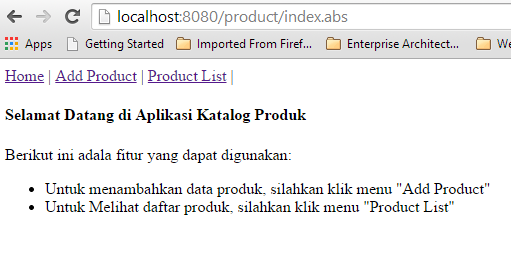
\includegraphics[width=0.6\textwidth]{img/hasil-index.png}
    \caption{Halaman web \texttt{index.html} yang dihasilkan}
    \label{fig:htmlIndex}
\end{figure}

\subsection{Komponen View \texttt{form.html}}
Halaman HTML ini berisikan \texttt{HTML Form} yang digunakan untuk memasukan data produk baru kedalam sistem. berikut ini adalah kode HTML yang harus dimasukan kedalam berkas \texttt{form.html} beserta gambar halaman web yang akan ditampilkan:

\begin{lstlisting}[
caption=Kode HTML untuk halaman \texttt{form.html},
label={lst:htmlProductForm},
]
<!DOCTYPE html>
<html>
	<head>
		<title>Add Product</title>
	</head>
<body>
	<div>
		<a href="/product/index.abs">Home</a> |
		<a href="/product/add.abs">Add Product</a> |
		<a href="/product/list.abs">Product List</a> |
	</div>
	<h3>Product Details</h3>
	<form method="POST" action="/product/saveData.abs">
	<table>
		<tbody>
			<tr>
				<td>Product SKU</td>
				<td>:</td>
				<td><input type="text" name="product_sku"/></td>
			</tr>
			<tr>
				<td>Product Name</td>
				<td>:</td>
				<td><input type="text" name="product_name"/></td>
			</tr>
			<tr>
				<td>Description</td>
				<td>:</td>
				<td><input type="text" name="description" /></td>
			</tr>
			<tr>
				<td>Price</td>
				<td>:</td>
				<td><input type="text" name="price" /></td>
			</tr>
		</tbody>
	</table>
	<input type="submit" value="Submit" />
	</form>
</body>
</html>
\end{lstlisting}

\begin{figure}
    \centering
    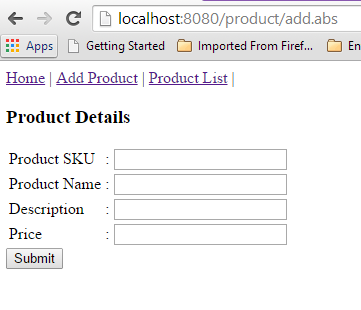
\includegraphics[width=0.6\textwidth]{img/hasil-add.png}
    \caption{Halaman web \texttt{form.html} yang dihasilkan}
    \label{fig:htmlForm}
\end{figure}

\subsection{Komponen View \texttt{update.html}}

HTML ini berfungsi untuk menampilkan data produk sesuai dengan \textit{input} (nomor SKU) yang diberikan. Melalui halaman ini juga, pengguna aplikasi dapat mengubah data produk tersebut sesuai dan kembali menyimpannya kedalam sistem. berikut ini adalah kode HTML yang harus dimasukan kedalam berkas \texttt{update.html} beserta gambar halaman web yang akan ditampilkan:

\begin{lstlisting}[
caption=Kode HTML untuk halaman \texttt{update.html},
label={lst:htmlUpdateProduct}
]
<!DOCTYPE html>
<html>
	<head>
		<title>Edit Product</title>
	</head>
<body>
	<div>
		<a href="/product/index.abs">Home</a> |
		<a href="/product/add.abs">Add Product</a> |
		<a href="/product/list.abs">Product List</a> |
	</div>
	<h3>Product Details: <span th:text="${data.sku}"></span></h3>
	<form method="POST" action="/product/saveUpdate.abs">
	<input type="hidden" name="product_sku" th:value="${data.sku}"/>
	<table>
		<tbody>
			<tr>
				<td>Product Name</td>
				<td>:</td>
				<td><input type="text" name="product_name" th:value="${data.name}"/></td>
			</tr>
			<tr>
				<td>Description</td>
				<td>:</td>
				<td><input type="text" name="description" th:value="${data.description}"/></td>
			</tr>
			<tr>
				<td>Price</td>
				<td>:</td>
				<td><input type="text" name="price" th:value="${data.price}"/></td>
			</tr>
		</tbody>
	</table>
	<input type="submit" value="Submit" />
	</form>
</body>
</html>
\end{lstlisting}

\begin{figure}
    \centering
    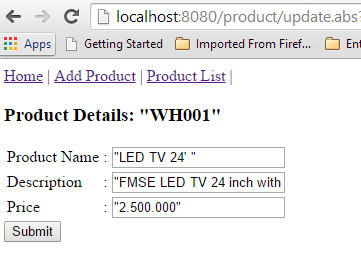
\includegraphics[width=0.6\textwidth]{img/hasil-update.png}
    \caption{Halaman web \texttt{update.html} yang dihasilkan}
    \label{fig:htmlUpdate}
\end{figure}

Seperti yang terlihat pada Kode \ref{lst:htmlUpdateProduct} di atas, penulis menambahkan sintaks Thymeleaf pada halaman ini agar halaman HTML ini dapat menampilkan data produk yang diberikan. Pada halaman ini, penulis menggunakan dua jenis sintaks Thymeleaf yaitu \texttt{th:text} dan \texttt{th:value}. sintaks \texttt{th:text} digunakan untuk menampilkan data dalam bentuk teks, sedangkan \texttt{th:value} adalah untuk menampilkan data kedalam bentuk atribut \texttt{value=""} di dalam tag \texttt{<input>}. Dengan menggunakan dua buah sintaks tersebut penulis sudah dapat menampilkan data produk pada halaman \texttt{update.html}.

\subsection{Komponen View \texttt{list.html}}

Halaman web ini dibuat dengan tujuan untuk menampilkan daftar seluruh produk yang disimpan di simpan oleh aplikasi dalam bentuk \texttt{HTML Table}. Berikut ini adalah kode HTML yang harus dimasukan kedalam berkas \texttt{list.html} beserta gambar halaman web yang akan ditampilkan:

\begin{lstlisting}[
caption=Kode HTML untuk halaman \texttt{list.html},
label={lst:htmlListProduct},
escapeinside={+}{+}
]
<!DOCTYPE html>
<html>
	<head>
		<title>Product List</title>
	</head>
<body>
	<div>
		<a href="/product/index.abs">Home</a> |
		<a href="/product/add.abs">Add Product</a> |
		<a href="/product/list.abs">Product List</a> |
	</div>
	<h3>Product List</h3>
	<table>
		<thead>
			<tr>
				<th>No.</th>
				<th>SKU</th>
				<th>Product Name</th>
				<th>Price</th>
				<th>Action</th>
			</tr>
		</thead>
		<tbody>
			<tr th:each="product: ${dataList}">
				<td th:text="${#ids.seq('')}"></td> +\label{lst:thymeSequence}+
				<td th:text="${product.sku}"></td>
				<td th:text="${product.name}"></td>
				<td th:text="${product.price}"></td>
				<td>
					<a th:href="@{http://localhost:8080/product/update.abs(sku=${product.sku})}">update</a>&nbsp;&nbsp; +\label{lst:thymeUrl}+
					<a th:href="@{http://localhost:8080/product/delete.abs(sku=${product.sku})}">delete</a> +\label{lst:thymeUrl2}+
				</td>
			</tr>
		</tbody>
	</table>
</body>
</html>
\end{lstlisting}

\begin{figure}
    \centering
    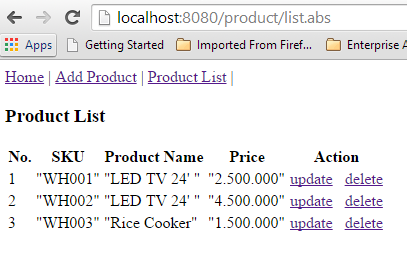
\includegraphics[width=0.6\textwidth]{img/hasil-list.png}
    \caption{Halaman web \texttt{list.html} yang dihasilkan}
    \label{fig:htmlList}
\end{figure}

Seperti yang terlihat pada Kode \ref{lst:htmlListProduct} diatas, penulis juga menambahkan sintaks Thymeleaf untuk dapat menampilkan data produk kedalam halaman web. Berbeda dengan Kode \ref{lst:htmlUpdateProduct} (halaman \texttt{update.html}) yang telah dibuat sebelumnya, pada halaman ini penulis menggunakan dua buah sintaks Thymeleaf yang lain yaitu \texttt{\$\{\#ids.seq()\}} (baris \ref{lst:thymeSequence}) dan \texttt{@\{url(param)\}} (baris \ref{lst:thymeUrl} dan \ref{lst:thymeUrl2}). Sintaks \texttt{\$\{\#ids.seq()\}} digunakan untuk menampilkan \textit{sequence id} seperti 1,2,3 dan seterusnya. Sedangkan sintaks \texttt{@\{url(param)\}} digunakan untuk menghasilkan URL dengan parameter seperti misalnya \texttt{http://localhost:8080/product/update.abs?sku=WH001}.

\section{Pembuatan Komponen Controller}

Setelah selesai membuat komponen View yang dibutuhkan, berikutnya adalah mengintegrasikan komponen Model dan View yang telah dibuat sebelumnya untuk menghasilkan sebuah halaman web yang utuh. Dalam proses pengembangan aplikasi web ini, penulis membuat sebuah modul Controller yang bernama \texttt{ProductController}. Untuk membuat komponen ini, penulis terlebih dahulu membuat sebuah modul baru yang bernama \texttt{ProductController} yang kemudian disimpan kedalam direktori \texttt{src/abs/controller} dengan nama \texttt{ProductController.abs}.\\

Berikut ini adalah konten dari modul \texttt{ProductController} yang penulis buat:

\begin{lstlisting}[
caption=Layout dari modul \texttt{ProductController},
label={lst:layoutProductController}
]
module Controller.Product;
import Product, ProductImpl from Model.Product;
import ABSHttpRequest from ABS.Framework.Http;
import ProductDB, ProductDBImpl from Model.ProductDB;

interface ProductController
{
	Pair<String, List<Product>> index(ABSHttpRequest request);
	Pair<String, List<Product>> addProduct(ABSHttpRequest request);
	Pair<String, List<Product>> saveDataProduct(ABSHttpRequest request);
	Pair<String, List<Product>> deleteProduct(ABSHttpRequest request);
	Pair<String, List<Product>> updateProduct(ABSHttpRequest request);
	Pair<String, List<Product>> saveUpdateProduct(ABSHttpRequest request);
	Pair<String, List<Product>> productList(ABSHttpRequest request);
}

class ProductControllerImpl implements ProductController
{
	//detail dari setiap method ada disini
}
\end{lstlisting}

Seperti yang terlihat pada Kode \ref{lst:layoutProductController} diatas, terdapat tujuan buah \textit{method} yang akan didefinisikan di dalam modul ini. Secara umum, ketujuh buah \textit{method} tersebut merupakan \textit{method} yang akan digunakan dalam proses \textit{create}, \textit{retrieve}, \textit{update} dan \textit{delete} produk pada aplikasi web yang dibuat. Berikut ini ada detail dari setiap \textit{method} yang ada di dalam modul \texttt{ProductController}:

\subsection{Method \texttt{index}}
Method ini digunakan untuk menampilkan halaman utama yang berisikan informasi singkat tentang aplikasi. Berikut ini adalah detail kode yang harus dibuat di dalam modul \texttt{ProductController}:

\begin{lstlisting}[
firstnumber=19,
caption=Detail kode ABS untuk \textit{method} \texttt{index},
label={lst:absProductIndex}
]
Pair<String, List<Product>> index(ABSHttpRequest request)
{
	return Pair("product/index", Nil);
}
\end{lstlisting}

Seperti yang terlihat pada Kode \ref{lst:absProductIndex} diatas, detail \textit{method} yang dibuat sangatlah sederhana yaitu hanya mengembalikan lokasi berkas HTML yang digunakan dengan tanpa adanya data yang  diberikan. Hal ini dilakukan karena halaman ini hanya merupakan halaman statis yang tidak membutuhkan data dari komponen Model untuk ditampilkan.

\subsection{Method \texttt{addProduct}}
Method ini digunakan untuk menampilkan halaman \texttt{form.html} berisikan \texttt{HTML Form} yang digunakan untuk mengirim data produk baru kepada aplikasi web. berikut ini adalah detail kode yang harus dibuat di dalam modul \texttt{ProductController}:

\begin{lstlisting}[
firstnumber=24,
caption=Detail kode ABS untuk \textit{method} \texttt{addProduct},
label={lst:absAddProduct}
]
Pair<String, List<Product>> addProduct(ABSHttpRequest request)
{
	return Pair("product/form", Nil);
}
\end{lstlisting}

Kode \ref{lst:absAddProduct} diatas secara umum mirip dengan \textit{method} \texttt{index} seperti yang tertera pada Kode \ref{lst:absProductIndex} sebelumnya. Method ini hanya mengembalikan lokasi berkas HTML yang digunakan dengan tanpa adanya data yang diberikan. 

\subsection{Method \texttt{saveDataProduct}}
Method ini digunakan untuk menerima dan menyimpan data produk yang dikirimkan oleh pengguna melalui halaman \texttt{form.html} dan kemudian menyimpannya kedalam \texttt{ProductDB} untuk kemudian ditampilkan kembali kedalam bentuk tabel. Berikut ini adalah detail kode ABS yang harus dibuat di dalam modul \texttt{ProductController}:

\begin{lstlisting}[
firstnumber=29,
caption=Detail kode ABS untuk \textit{method} \texttt{saveDataProduct},
label={lst:absSaveDataProduct},
escapeinside={@}{@}
]
Pair<String, List<Product>> saveDataProduct(ABSHttpRequest request)
{
	ProductDB db = new local ProductDBImpl();
	db.init(); @\label{lst:absInitDB}@
	
	String sku = request.getInput("product_sku"); @\label{lst:absGetInput}@
	String name = request.getInput("product_name");
	String description = request.getInput("description");
	String price = request.getInput("price"); @\label{lst:absGetInput2}@
	
	Product p = new local ProductImpl(sku, name, description, price);
	db.save(p);
	
	List<Product> dataList = db.findAll();
	return Pair("product/list", dataList);
}
\end{lstlisting}

Seperti yang terlihat pada Kode \ref{lst:absSaveDataProduct} diatas, penulis membuat objek \texttt{ProductDB} yang sudah dibuat sebelumnya pada tahap pembuatan komponen Model. objek ini berfungsi sebagai tempat penyimpanan data produk sementara untuk mensimulasikan proses \textit{create}, \textit{retrieve}, \textit{update} dan \textit{delete}. Setelah membuat objek dari \texttt{ProductDB}, berikutnya penulisan melakukan proses inisialisasi data dengan memanggil \textit{method} \texttt{init} (lihat Kode \ref{lst:absInitDB}). Tujuan dari pemanggilan ini adalah untuk mengisi \texttt{ProductDB} dengan data \textit{dummy} sebagai data awalan yang dimiliki oleh aplikasi.\\

Setelah proses initialisasi \texttt{ProductDB} selesai, berikutnya adalah menangkap input yang diberikan oleh pengguna melalui objek \texttt{ABSHttpRequest}. Untuk dapat mengakses HTTP POST atau GET data yang diberikan oleh \textit{web server} penulis menggunakan \textit{method} \texttt{getInput} yang dimiliki oleh objek \texttt{ABSHttpRequest} seperti yang terlihat pada Kode \ref{lst:absGetInput} sampai \ref{lst:absGetInput2}). Setelah berhasil mengambil \textit{input} dari \textit{web server} selanjutnya penulis membuat sebuah objek \texttt{Product} baru yang kemudian disimpan kedalam objek \texttt{ProductDB}. Sampai pada tahap ini, data produk baru yang dibuat sudah masuk kedalam objek \texttt{ProductDB} dan untuk membuktikannya penulis menampilkan seluruh data produk yang disimpan kedalam halaman web \texttt{list.html}

\subsection{Method \texttt{deleteProduct}}
Method ini digunakan untuk menghapus data produk yang ada di dalam \texttt{ProductDB} berdasarkan nomor sku yang diberikan. Berikut ini adalah detail kode ABS yang harus dibuat di dalam modul \texttt{ProductController}:

\begin{lstlisting}[
firstnumber=46,
caption=Detail kode ABS untuk \textit{method} \texttt{deleteProduct},
label={lst:absDeleteProduct},
escapeinside={@}{@}
]
Pair<String, List<Product>> deleteProduct(ABSHttpRequest request)
{
	ProductDB db = new local ProductDBImpl();
	db.init();
	
	String sku = request.getInput("sku");@\label{lst:absGetInputSKU}@
	Product p = db.findBySku(sku); @\label{lst:absFindBySKU}@
	db.delete(p); @\label{lst:absCallDelete}@
	
	List<Product> productList = db.findAll();
	return Pair("product/list", productList);
}
\end{lstlisting}

Seperti yang terlihat pada Kode \ref{lst:absDeleteProduct} bais \ref{lst:absGetInputSKU}, penulis mengambil \textit{input} dari pengguna berupa nomor sku dari produk yang dipilih. Dengan menggunakan nomor sku yang diberikan, penulis mencoba untuk mendapatkan object \texttt{Product} yang tersimpan di dalam \texttt{ProductDB} (lihat Kode \ref{lst:absFindBySKU}). Setelah objek \texttt{Product} yang diinginkan telah berhasil diperoleh, berikunya penulis menghapus produk tersebut dari dalam \texttt{ProductDB} (lihat Kode \ref{lst:absCallDelete}). Dengan menggunakan cara ini, penulis telah mensimulasikan proses penghapusan data yang tersimpan di dalam aplikasi berdasarkan \textit{input} yang diberikan oleh pengguna.
 
\subsection{Method \texttt{updateProduct}}

Method ini digunakan untuk menampilkan detail produk yang dipilih untuk kemudian diubah datanya dan disimpan kembali kedalam aplikasi. Halaman detail produk yang digunakan pada \textit{method} ini adalah halaman \texttt{update.html} yang berisikan \texttt{HTML Form} untuk dapat mengirimkan data perubahan kepada modul \texttt{ProductController}. Berikut ini adalah kode ABS yang harus dibuat di dalam modul \texttt{ProductController}:

\begin{lstlisting}[
firstnumber=59,
caption=Detail kode ABS untuk \textit{method} \texttt{updateProduct},
label={lst:absUpdateProduct},
escapeinside={@}{@}
]
Pair<String, List<Product>> updateProduct(ABSHttpRequest request)
{
	ProductDB db = new local ProductDBImpl();
	db.init();
	
	String sku = request.getInput("sku");
	Product p = db.findBySku(sku);
	
	List<Product> products = Nil;
	products = appendright(products, p);
	
	return Pair("product/update", products);
}
\end{lstlisting}

Seperti yang terlihat pada Kode \ref{lst:absUpdateProduct} diatas, penulis mencoba mengambil \textit{input} berupa nomor sku yang dikirimkan oleh \textit{web browser}. Setelah mendapatkan nomor sku yang diberikan, selanjutnya penulis melakukan pencarian data produk dengan memanggil \textit{method} \texttt{findBySku} milik \texttt{ProductDB}. Setelah berhasil mendapatkan data yang diinginkan, selanjutnya adalah memberikan data tersebut kepada \textit{web server} untuk kemudian ditampilkan pada halaman \texttt{update.html}.

\subsection{Method \texttt{saveUpdateProduct}}

Method ini digunakan untuk menyimpan perubahan data produk yang diberikan oleh pengguna melalui halaman \texttt{update.html} dan kemudian menampilkan kembali seluruh data yang kedalam halaman \texttt{list.html}. Berikut ini adalah detail kode ABS yang harus dibuat di dalam modul \texttt{ProductController}:

\begin{lstlisting}[
firstnumber=73,
caption=Detail kode ABS untuk \textit{method} \texttt{saveUpdateProduct},
label={lst:absSaveUpdateProduct},
escapeinside={@}{@}
]
Pair<String, List<Product>> saveUpdateProduct(ABSHttpRequest request)
{
	ProductDB db = new local ProductDBImpl();
	db.init();
	
	String sku = request.getInput("product_sku");
	String name = request.getInput("product_name");
	String description = request.getInput("description");
	String price = request.getInput("price");
	
	Product p = db.findBySku(sku); @\label{lst:updateDataProduct}@
	p.setName(name);
	p.setDescription(description);
	p.setPrice(price);
	db.update(p); @\label{lst:updateDataProduct2}@
	
	List<Product> products = db.findAll();
	return Pair("product/list", products);
}
\end{lstlisting}

Seperti yang terlihat pada Kode \ref{lst:absSaveUpdateProduct} baris \ref{lst:updateDataProduct} sampai \ref{lst:updateDataProduct2}, penulis melakukan pencarian data produk di dalam \texttt{ProductDB} sesuai dengan nomor sku yang diberikan. Setelah data produk yang diminta berhasil ditemukan, selanjutnya adalah mengubah data-data pada produk tersebut sesuai dengan \textit{input} yang diberikan oleh pengguna dan menyimpannya kembali kedalam \texttt{ProductDB}. Untuk membuktikan perubahan yang dilakukan penulis menampilkan seluruh data yang ada di dalam modul \texttt{ProductDB} kedalam halaman \texttt{list.html}.

\subsection{Method \texttt{productList}}
Method ini digunakan untuk menampilkan seluruh data yang tersimpan di dalam \texttt{ProductDB} kedalam halaman \texttt{list.html}. Berikut ini adalah detail kode ABS yang harus dibuat di dalam modul \texttt{ProductController}:

\begin{lstlisting}
firstnumber=93,
caption=Detail kode ABS untuk \textit{method} \texttt{productList},
label={lst:absProductList}
]
Pair<String, List<Product>> productList(ABSHttpRequest request)
{
	ProductDB db = new local ProductDBImpl();
	db.init();
	
	List<Product> productList = db.findAll();
	return Pair("product/list", productList);
}
\end{lstlisting}

\section{Pemetaan URL dengan Komponen Controller}

Setelah selesai membuat komponen Model, View dan Controller yang dibutuhkan, langkah selanjutnya adalah memetakan setiap alamat URL yang akan diakses dengan \textit{method} telah dibuat pada komponen \texttt{ProductController}. Proses pemetaan URL tersebut dapat dilakukan dengan cara menuliskan daftar URL yang akan diakses beserta nama komponen Controller dan \textit{method}-nya kedalam modul \texttt{RouteConfig} yang berada di dalam berkas \texttt{src/abs/framework/Route.abs}. Berikut ini adalah detail kode ABS yang harus dimasukkan kedalam modul tersebut.

\begin{lstlisting}[
caption=Detail kode ABS untuk mendefinisika pemetaan URL,
label={lst:absRouteConfig}
]
module ABS.Framework.Route;

interface RouteConfig
{
	String route(String url);
}

class RouteConfigImpl implements RouteConfig
{
	String route(String url)
	{
		String result = case url
		{
			"/product/index.abs" => "Controller.Product.ProductControllerImpl@index";
			"/product/add.abs" => "Controller.Product.ProductControllerImpl@addProduct";
			"/product/saveData.abs" => "Controller.Product.ProductControllerImpl@saveDataProduct";
			"/product/delete.abs" => "Controller.Product.ProductControllerImpl@deleteProduct";
			"/product/update.abs" => "Controller.Product.ProductControllerImpl@updateProduct";
			"/product/saveUpdate.abs" => "Controller.Product.ProductControllerImpl@saveUpdateProduct";
			"/product/details.abs" => "Controller.Product.ProductControllerImpl@productDetails";
			"/product/list.abs" => "Controller.Product.ProductControllerImpl@productList";
			_ => "";
		};
		
		return result;
	}
}
\end{lstlisting}

Sampai pada tahap ini, penulis telah membuat komponen Model, View dan Controller beserta pemetaan URLnya. Hal yang dilakukan selanjutnya adalah melakukan proses kompilasi dan \textit{deployment} dengan menggunakan \textit{build script} yang sudah tersedia. Untuk dapat menjalankan kedua proses tersebut, penulis terlebih dahulu membuka Terminal Console (misal: Command Prompt pada Windows) yang ada di dalam komputer milik penulis dan kemudian masuk kedalam direktori ABS MVC Framework. Setelah masuk kedalam direktori ABS MVC Framework selanjutnya penulis menjalankan \textit{build script} (\texttt{build.xml}) yang tersedia di dalam direktori tersebut dengan mengetikan perintah \texttt{ant -Dabsproduct=Default abs.deploy}.\\

Setelah aplikasi web yang dibuat berhasil di\textit{compile} dan di\textit{deploy} kedalam ABS Server, berikutnya adalah menjalankan ABS Server yang sudah tersebut melalui Terminal Console dengan cara masuk kedalam direktori ABS Server dan menjalankan perintah \texttt{java -jar absserver.jar}. Setelah ABS Server-nya berhasil dijalankan, aplikasi web yang telah dibuat sebelumnya dapat diakses dengan mengetikan alamat \texttt{http://localhost:8080/product/index.abs}.


